\documentclass[german,12pt,doc]{apa}
\usepackage[a4paper, left=25mm, right=40mm]{geometry}
\usepackage{apacite}
\usepackage{amsmath}
\usepackage[german]{babel}
\usepackage{epstopdf} 
\usepackage{verbatim}
\usepackage{float}
\usepackage[firstpage]{draftwatermark}
\SetWatermarkScale{4}
\SetWatermarkText{Entwurf}
\SetWatermarkLightness{0.8}
\usepackage{setspace}
\usepackage{graphicx}

\usepackage{caption}
\usepackage{prettyref}

\usepackage[nonumberlist,sanitize={name=false}]{glossaries}
\makeglossaries

\onehalfspacing
\setlength{\parskip}{1em} % 1ex plus 0.5ex minus 0.2ex}
\setlength{\parindent}{0pt}

\usepackage[utf8]{inputenc}


\usepackage[]{blindtext}
\rightheader{Automatisierte Verfahren zur Prädiktorauswahl}
% Hurenkinder und Schusterjungen verhindern
\clubpenalty10000
\widowpenalty10000
\displaywidowpenalty=10000

\begin{document}

\title{Automatische Verfahren zur Prädiktorauswahl in Regressionsmodellen}
\shorttitle{Prädiktorauswahl in Regressionsmodellen} 
\author{Literaturarbeit vorgelegt von \\ Markus Graf (markus.graf@uzh.ch)}
\date{\today}
\affiliation{am  Psychologisches Institut der Universität Zürich\\ Betreut durch Dr. Christina Werner\\ \today}
\abstract{Ziel der multiplen Regression ist es Kriteriumsvariablen durch mehrere Prädiktorvariablen möglichst gut vorherzusagen. In diesem Kontext kommen Automatische Modellwahlverfahren zur Anwendung, wenn für die Schätzung des Modells viele potentielle Prädikatoren zur Auswahl stehen, insbesondere wenn theoretische Grundlagen fehlen. Das exhaustive Verfahren in Kombination mit der Kreuzvalidierung ist momentan die einzige Technik, die das beste und stabilste Modell findet. Schrittweise Verfahren kommen zur Anwendung bei kleinem Stichprobenumfang. Während früher aus Mangel an Rechenleistung standardmässig schrittweise Verfahren angewandt wurden soll heutzutage dem rechenintensiven exhaustiven Verfahren bevorzugt werden.
}
\maketitle
\begin{center}

\includegraphics[width=0.1\textwidth]{cc_by_sa.jpg}\\
Dieses Werk bzw. Inhalt steht unter einer Creative Commons Namensnennung - Weitergabe unter gleichen Bedingungen 3.0 Unported Lizenz.
\end{center}
\setlength{\parindent}{0pt}
\newpage
\tableofcontents
\newpage

\newglossaryentry{glos:rechenaufwand}{name=Rechenaufwand, description={ beschreibt die Komplexität eines Verfahrens. Die Anzahl der Schritte, die für die Berechnung benötigt werden, dient als Kennzahl}} 

\newglossaryentry{glos:trainingsdatensatz}{name=Trainingsdatensatz, description={liefert die Datenbasis für die Schätzung der Modellparameter}} 

\newglossaryentry{glos:datamining}{name=Datamining,description={Systematische Anwendung statistischer Methoden auf einen grossen Datenbestand mit dem Ziel, neue Muster zu erkennen}}

\newglossaryentry{glos:praediktorvariable}{ plural={Prädiktorvariablen},name=Prädiktorvariable,description={Unabhängige Variable, die einen zu bestimmenden Einfluss auf die Kriteriumsvariable ausübt}}

\newglossaryentry{glos:kriteriumsvariable}{name=Kriteriumsvariable,description={Erklärte Variable, welche eine Wirkung misst}}

\newglossaryentry{glos:kreuzvalidierung}{name=Kreuzvalidierung,description={ bezeichnet Verfahren, bei denen die Vorhersagezuverlässigkeit eines Modells anhand von unabhängigen Teilstichproben bestimmt wird}}

\newglossaryentry{glos:exhaustive Verfahren}{name=exhaustive Verfahren,plural={exhaustiven Verfahren},description={ rechnen alle möglichen Modelle anhand der potentiellen Prädiktoren durch}}

\newglossaryentry{glos:schrittweise Verfahren}{name=schrittweise Verfahren,description={rechnen Modelle durch  schrittweise Hinzunahme beziehungsweise Weglassen potentieller Prädiktoren}}

\newglossaryentry{glos:Modellguete}{name=Modellgüte,description={beschreibt, wie gut ein Modell gegebene Daten vorhersagen kann}}

\newglossaryentry{glos:Overfitting}{name=Overfitting,description={beschreibt eine mangelnde Generalisierbarkeit aufgrund eines Modells, das zu sehr an die Trainingsstichprobe angepasst ist}}

\newglossaryentry{glos:Multikollinearitaet}{name=Multikollinearität,description={ ist ein Problem der Regressionsanalyse und liegt vor, wenn zwei oder mehr Prädiktoren stark miteinander korrelieren}}

\newglossaryentry{glos:Stabilitaet}{name=Stabilität,description={beschreibt, wie stark die Vorhersagen eines Modells im Generellen variieren}}

\newglossaryentry{glos:Maximum-Likelihood-Methode}{name=Maximum-Likelihood-Methode,description={ wird benützt, um die unbekannten Parameter einer Funktion aus gemessenen Daten zu bestimmen}}

\section{Einführung}
Das Standardverfahren um eine \Gls{glos:kriteriumsvariable} durch \Glspl{glos:praediktorvariable} vorherzusagen stellt die Regressionsanalyse dar.
Begründet wurde dieses Verfahren durch Carl Friedrich Gauss in seiner Schrift, in der er, mit Hilfe der Methode der kleinsten Quadrate, die Bewegung der Himmelskörper um die Sonne im Kegelschnitt beschrieb \cite{gauss1809theoria}. 

Im Unterschied zur einfachen linearen Regression, werden in einem multiplen Regressionsmodell mehrere Prädiktoren $p$ mit einbezogen. 
Es resultiert eine Regressionsgleichung welche zur Vorhersage einer Kriteriumsvariable aufgrund mehrerer Prädikatorvariablen genutzt wird  \cite[S. 448]{bortz2011}. 
\begin{equation}
x_i = \beta_0 + \beta_1\cdot x_{i1} + ... +  \beta_p\cdot x_{ip} + \epsilon_i
\tag{multiple lineare Regression}
\end{equation}
Beim klassisch hypothesengeleiteten Vorgehen wird eine Hypothese definiert, welche empirisch getestet wird.
Der empirische Test wiederum ist ein Modell, in unserem Fall eine Regressionsgleichung, welches aufgrund theoretischer Überlegungen erstellt wurde.
Wenn es jedoch keine klaren theoretischen Gründe gibt potentielle in Frage kommende Prädiktorvariablen in das Modell auf zu nehmen werden mehrere Modelle geschätzt und das mit der besten und stabilsten Vorhersagekraft verwendet.
Bei komplexen Modellen mit vielen Prädiktoren werden Modelle mittels automatischer Verfahren geschätzt und selektiert.
Ein zentrales Problem solcher Verfahren ist, dass sie dazu neigen zu komplexe Modelle zu schätzen. 
Komplexe Modelle können sehr gute Vorhersagen liefern innerhalb des Trainingsdatensatz, doch oft scheitern die Vorhersage beim Versuch, diese zu generalisieren.  

Im folgenden wird diskutiert wann und weshalb automatische Verfahren zur Modellwahl eingesetzt werden. 
Anschliessend wird das exhaustive und schrittweise Verfahren vorgestellt und kritisch diskutiert.
Die Frage nach der Generalisierbarkeit atomatisch geschätzter Modelle wird im Anschluss besprochen und die Kreuzvalidierung als Lösungsansatz genannt.
\section{Recherche}
Hauptquelle der Literatur-Recherche waren Artikel, welche via Google Scholar gefunden wurden. Grundlagen zu den Verfahren wurden mittels \citeA{bortz2011} und \citeA{jacob2003applied} erarbeitet. Der Fokus bei der Recherche wurde auf Artikel im Bereich der Psychologie gerichtet, es fanden sich jedoch auch  viele Artikel in anderen Fachbereichen, welche mit den selben Problemen konfrontiert sind. Kurz vorgestellt wurden die Verfahren von Carolin Strobl in der Vorlesung ``160 Psychologische Methoden: Datenerhebung, Analyse und Darstellung'' im Rahmen des Psychologie-Aufbaustudiums der Universität Zürich. Interessante Hinweise und praktische Beispiele fanden sich ausserdem in den Manuals von R.
\section{Sinn und Zweck automatisierter Modellwahl}
In psychologischen Fragestellungen kommt es vor, dass viele Prädiktoren in ein Modell einfliessen oder potentiell für ein Modell in Frage kommen.
Die Frage, welche Prädiktoren nun ein Modell am besten beschreiben ist dabei die eigentliche Gretchenfrage. 

Unterteilen lässt sich die automatisierte Modellwahl in (a) eine explorative, und (b) eine optimierende Anwendung. 

Im Falle der explorativen Anwendung fehlen grösstenteils theoretische Begründungen für die Auswahl bestimmter Prädiktoren. Ein Beispiel für eine solche Anwendung liefert eine Studie, die Prädiktoren des Alltagstransfers eines stationär erlernten Entspannungstrainings suchte \cite{023755520080101}.
Oft werden Daten gleich für mehrere Studien erhoben und in anderen Studien verwendet.
Diese systematische Anwendung automatischer Modellwahlverfahren, mit dem Ziel neue Muster zu erkennen, ist damit eine Aufgabenstellung des Datamining. 
Die so gewonnen Daten können zu neuen Fragestellungen führen. 

Der zweite Anwendungsfall ergibt sich, wenn bereits ein Modell vorhanden ist. Insbesondere komplexe Modelle sind meist schlecht generalisierbar. Automatisierte Verfahren können  helfen, Prädiktoren zu erkennen, welche die Komplexität unnötig erhöhen.
\section{Automatische Verfahren zur Prädiktorauswahl}
Zu Beginn der psychologischen Forschung mussten Modelle von Hand berechnet werden. Zwangsläufig wurden wenige Prädiktoren erhoben und einfache Modelle gerechnet. 
Friedman analysierte beispielsweise 1944 die Langlebigkeit von Turbinenschaufeln in Abhängigkeit von Stress, Temperatur und einigen Legierungsparametern. 
Zwar wurde die Berechnung nicht mehr von Hand durchgeführt, doch benötigte eine Regressionsschätzung inklusive Berechnung der Teststatistiken rund 40 Stunden \cite[p.2]{armstrong2011illusions}. Jeder durchschnittliche Computer erledigt dies heutzutage in Sekundenbruchteilen. 
Mit dem technischen Fortschritt einhergehend wurden Verfahren entwickelt, welche alle möglichen Kombinationen von Prädiktoren, inklusive ihrer Interaktionen, berücksichtigen und gegeneinander testen.

Es gilt also, das ``beste'' Modell zu schätzen. 
Gemeint ist mit dem ``besten'' Modell das, das innerhalb des Trainingsdatensatzes die beste Vorhersage liefert. 
Anhand des Trainingsdatensatzes wurde das Modell jedoch auch geschätzt. Entsprechend kann es Modelle geben, die in der Gesamtpopulation bessere Vorhersagen liefern. 
``All models are wrong, but some are useful'' \cite[p.424]{box1979robustness}.
Box will damit hervorheben, dass obschon in der Literatur oft vom ``besten'' oder ``wahren'' Modell gesprochen wird, dies nur eine Approximation der Wirklichkeit darstellt \cite[p.172]{weakliem2004introduction}.

\subsection{Exhaustive Schätzung}
Eine naive Herangehensweise ist, alle möglichen Modelle durchzurechnen, welche mit $p$ Prädiktoren möglich sind. 
Zur Beurteilung der Modellgüte kann die mittlere quadratische Abweichung herangezogen werden.
Das Modell mit der kleinsten Fehlerquadratsumme $SSE_p$ wird als das  optimale Modell bezeichnet \cite[p. 6]{thompson1978selection}. 

\begin{equation}
SSE_p = \sum_{i=1}^n(y_{ip}-\hat y_{p})^2
\tag{Fehlerquadratsumme}
\end{equation}


Da alle möglichen Kombinationen durchgerechnet werden, wird das  Modell gefunden, das den Trainingsdatensatz am besten vorhersagt.
\citeA[p.6]{thompson1978selection} sieht einzig den Nachteil darin, dass der \Gls{glos:rechenaufwand} exponentiell mit der Anzahl zu berücksichtigender Prädiktoren steigt. 
Es müssen immer $2^p-1$ Modelle berechnet werden: Bei 5 Prädiktoren sind dies 31 Modelle, bei 10 bereits 1023 usw.
Während früher eingeschränkte Rechenkapazität oft ein ökonomischer Faktor war -- es musste Rechenzeit in einem Rechenzentrum reserviert werden -- spielt die Rechengeschwindigkeit auf modernen Systemen eine untergeordnete Rolle. 
%In der psychologischen Forschung muss oft nur eine Handvoll Prädiktoren in die Schätzung einbezogen werden.

\subsection{Schrittweise Verfahren} 
Das optimale Modell beinhaltet jeden Prädiktor, der die Voraussage auch nur minimal verbessert. 
Es stellt sich die Frage, ob diese minimale Verbesserung auch nützlich ist oder einfach durch Zufall entstanden ist. 
Schrittweise Verfahren arbeiten wesentlich liberaler.  Prädiktoren werden hinzugefügt oder eliminiert, je nach deren Relevanz für die Modellgüte. 
Es werden Kriterien festgelegt, nach welchen ein Modell als angemessen zu betrachten ist. 
Dies hat gegenüber dem \glspl{glos:exhaustive Verfahren} den Vorteil, dass nicht alle Modelle berechnet werden müssen und entsprechend schneller Lösungen gefunden werden.

Innerhalb der schrittweisen Verfahren unterscheidet man zwischen \textit{Forward Selection} und \textit{Backward Elimination}. 
\begin{figure}[htbp]
	\centering
	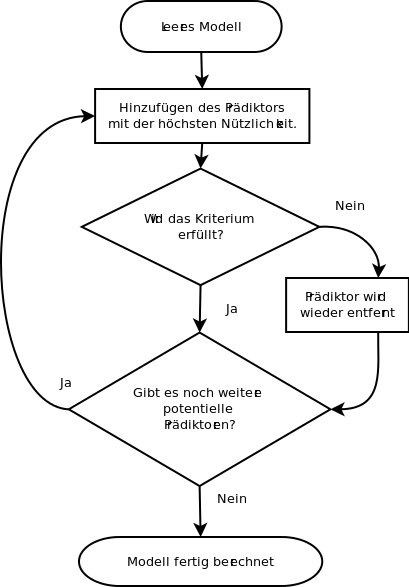
\includegraphics[height=0.5\textheight]{forward_stepwise.png}
	\caption{Forward Selection. Das Flussdiagramm beschreibt den schrittweisen Aufbau eines neuen Modells aus dem leeren Modell durch Hinzufügen potentieller Prädiktoren.}
	\label{fig:forward_stepwise}
	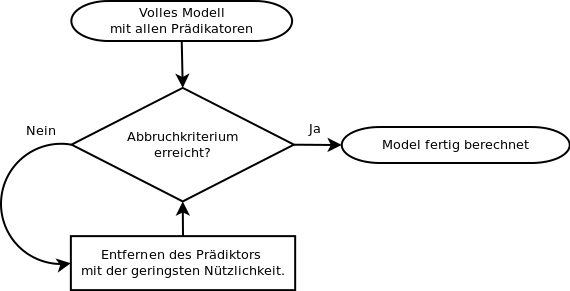
\includegraphics[height=0.5\textheight]{backward_stepwise.png}
	\caption{Backward Elimination. Das Flussdiagramm beschreibt die schrittweise Elimination von unnützen Prädiktoren aus dem vollen Modell.}
	\label{fig:backward_stepwise}
\end{figure}
Ausgehend vom leeren Modell werden in der ersten Variante schrittweise weitere Variablen der Nützlichkeit nach in das Modell integriert. Dies dauert so lange an, bis kein Prädiktor mehr gefunden wird, der ein gewisses Kriterium erfüllt.

In der zweiten Variante werden alle Prädiktoren in das Modell integriert und sukzessive nacheinander entfernt. Wiederum endet das Verfahren, sobald kein Prädiktor mehr weggelassen werden kann, ohne dass ein gewisses Kriterium unterschritten wird.

Die Aufnahme einer neuen Variable kann dazu führen, dass eine bereits im Modell vorhandene Variable obsolet wird. 
Um diesem Umstand Rechnung zu tragen, werden oft Forward Selection und Backward Elimination kombiniert \cite[p. 461]{bortz2011}. 

In seltenen Fällen kann es vorkommen, dass zwei Variablen für sich in die Regressionsgleichung aufgenommen, die Vorhersage kaum verbessern und das Kriterium nicht erfüllen. Zusammen leisten sie jedoch  einen substantiellen Beitrag \cite[p.261]{jacob2003applied}. 
\Gls{glos:schrittweise Verfahren} mittels Forward Selection sind entsprechend nicht in der Lage solche Effekte mit zu berücksichtigen, wogegen Backward Elimination robuster gegen solche Supressionseffekte ist \cite{shieh2006suppression}. 

Zentrales Element der schrittweisen Regression ist das Kriterium zur Beurteilung der  Modellanpassung, welches besagt, weshalb und wann ein Modell als akzeptabel zu betrachten ist. Als Folge dessen, wird damit auch die Anzahl relevanter Prädiktoren bestimmt. Im Laufe der Zeit wurden diverse Kriterien definiert, welche alle für sich ihre Berechtigung haben.
Einteilen lassen sie sich in Kriterien, welche (a) sich auf die Beurteilung innerhalb des Trainingsdatensatzes beschränken oder (b) die Generalisierbarkeit ausserhalb des Trainingsdatensatzes zu berücksichtigen versuchen. Letztere werden im Abschnitt des Overfittings beschrieben.

Interessiert uns die \Gls{glos:Modellguete} innerhalb des Trainingsdatensatzes bietet das Bestimmtheitsmass erste Hinweise. Im Fall der multiplen Regression entspricht dies dem Quadrat des multiplen Korrelationskoeffizienten $R^2$ und  besagt, wie viel systematische Varianz durch das Modell aufgeklärt  wird. 
Das Bestimmtheitsmass steigt mit der Anzahl der Prädiktoren $p$, insbesondere bei kleinem Stichprobenumfang $n$, weshalb eine Schrumpfungskorrektur vorgenommen werden muss \cite[p. 451]{bortz2011}. 

\begin{equation}
\bar R^2=1-\frac{\displaystyle \frac{1}{n-p-1} \sum_{i=1}^n (Y_i-\hat{Y}_i)^2}{\displaystyle \frac{1}{n-1} \sum_{i=1}^n (Y_i-\bar{Y})^2}
\tag{korrigiertes Bestimmtheitsmass}
\end{equation}

In schrittweisen Verfahren wird nicht einzig aufgrund von $R^2$ selektiert, sondern es wird zusätzlich getestet, ob Verbesserungen nicht durch Zufall entstanden sind. 

Beim Signifikanztest als Kriterium wird das Verfahren beendet, wenn kein Prädiktor mehr hinzugefügt werden kann, der das Vorhersagepotential signifikant erhöht \cite[p.48]{bendel1977comparison}. 
Das Vergleichen zweier Regressionsgleichungen mittels Signifikanztest bedingt, dass diese geschachtelt sein müssen, das heisst, das kleinere Modell muss im grösseren enthalten sein \cite[p. 508]{jacob2003applied}.
Das gewählte Signifikanzniveau ist eigentlich arbiträr gewählt und eher als Konvention zu betrachten. Das Signifikanzniveau soll grundsätzlich die relativen Kosten der Irrtumswahrscheinlichkeit beschreiben \cite[p. 196]{hansen1999discussion}. \citeA[p. 269]{derksen2011backward} diskutieren mehrere Empfehlungen für Signifikanzniveaus und weisen darauf hin, das sich über mehrere Tests der $\alpha$-Fehler kumuliert. 
In  Simulationen mit artifiziellen Daten zeigen \citeA{mundry2009stepwise} das  Problem multipler Tests beispielhaft auf. 
Daraus resultierend lehnen sie die Verwendung der schrittweisen Regression mittels Signifikanztest gar ab.

Eine weitere Schwäche des Hypothesentestens ist der Einfluss der Stichprobengrösse. So kann bei genügend grossem Umfang nahezu jedes Modell  signifikant werden, was wiederum zu komplexen und überangepassten Modellen führt \cite[p.173]{weakliem2004introduction}.

Entgegen dem exhaustiven besteht bei schrittweisen Verfahren das Problem, dass unter Umständen nicht das optimale Modell gefunden wird. 
\citeA[p. 462]{bortz2011} bezeichnen diese Verfahren eher als explorativ, da die Nützlichkeitsunterschiede, die oft nur geringe statistische Bedeutung haben, das Modell bestimmen.
\citeA[p. 56ff]{harrell2001regression} lehnt das Verfahren gar ab und führt ins Feld, dass sämtliche statistischen Prinzipien verletzt würden. 
\citeA{berk1978comparing} zeigte in einem Vergleich, dass die durchschnittliche Differenz der Fehlerquadratsummen zwischen exhaustiver und schrittweiser Regression kaum 7\% übertrifft. Bei Modellen, welche im Allgemeinen bereits viel Varianz aufklären, mag dies akzeptabel sein. Wenn hingegen zu befürchten ist, dass wenig Varianz aufgeklärt werden kann, könnte diese Differenz jedoch das Zünglein an der Waage sein.
\section{Multikollinearität}
\Gls{glos:Multikollinearitaet}, als hohe Korrelationen zwischen mehreren Prädikatoren, führt zu Problemen bei der automatischen Modellwahl. 
In schrittweisen Verfahren ist es in solchen Fällen häufig vom Zufall abhängig welche der beteiligten Variablen als erste weggelassen beziehungsweise aufgenommen wird. 
Ein Anstieg der Korrelation zwischen Prädiktoren hat zur Folge, dass (a) die p-Werte bei Signifikanztests sinken, (b) schwache Prädiktoren entgegen den starken eher fälschlicherweise ausgeschlossen werden, (c) korrekt hoch signifikante Prädiktoren werden eher ausgeschlossen wenn die Korrelation zwischen einem konfundierenden Prädikator und dem Kriterium steig und (d) selbst wenn die Korrelation zwischen konfundierendem Prädikator und Kriterium klein ist, besteht die Gefahr, dass korrekt schwach signifikante Prädiktoren nicht signifikant werden \cite[p. 2810]{graham2003confronting}.

Grundsätzlich gilt die Unabhängigkeit der Prädikatoren als Voraussetzung für die multiple Regression. Doch gerade in der psychologischen Forschung lassen sich Korrelationen meist schlecht vermeiden.
Um bereits im Vorfeld Hinweise auf potentielle Kollinearität zu erhalten, empfiehlt es sich die Kovarianzmatrix zwischen allen Prädikatoren vor der eigentlichen Auswahl zu betrachten.
Eventuell wurde das selbe Merkmal mehrmals erhoben.
Der Zusammenhang zwischen einer Prädikatorvariable $i$ und der vorhergesagten Kriteriumsvariable lässt sich mit dem Strukturkoeffizienten $c_i$ ausdrücken.
\begin{equation}
c_i = \frac{r_{ic}}{R}
\tag{Strukturkoeffizient}
\end{equation}
$r_{ic}$ beschreibt den einzelnen Korrelationskoeffizient zwischen dem Prädikator $i$ und dem Kriterium $c$ und $R$ den multiplen Korrelationskoeffizient. 
So kann auf die Prädikatoren eingeschränkt werden,  welche am besten das Kriterium vorhersagen \cite[S. 453]{bortz2011}. 

\section{Overfitting}
Es können beliebig viele potentiell erklärende Variablen erhoben werden, um sich komplexe Modelle generieren zu lassen. 
Und Menschen tendieren zu glauben, dass komplexe Probleme komplexe Lösungen benötigen. 
Die Forschung zeigt jedoch, dass oft das Umgekehrte der Fall ist \cite[p.3]{armstrong2011illusions}. 
Insbesondere Gigerenzer demonstrierte eindrucksvoll, wie mit einfachen Rekognitionsheuristiken bessere Vorhersagen gemacht werden konnten als mit komplexen statistischen Modellen \cite{borges1999can}.
Komplexe Modelle können sehr gute Vorhersagen innerhalb des Trainingsdatensatzes liefern, doch  scheitern oft beim Versuch der Generalisierung.  

Die Illusion der Komplexität ist auch in der Statistik anzutreffen \cite[p. 3]{armstrong2011illusions}. 
Im Kontext der Modellwahl äussert sich dies in Form des  \Gls{glos:Overfitting}s. Das heisst, dass das Modell zu sehr an den Trainingsdatensatz angepasst ist.
Insbesondere Modellwahlverfahren, welche die Anzahl der Prädikatoren nicht bestrafen, sind davon betroffen.
Als Einflussfaktoren seitens der Daten sind Repräsentativität und Stichprobengrösse zu nennen. 
Mit steigendem Stichprobenumfang und höherer Repräsentativität sinkt das Overfitting und steigt die Stabilität der Vorhersage.

\subsection{Kriterienbasierte Strategien}
Die bisher beschriebenen Modellwahlverfahren fokussieren sich darauf, anhand der gegebenen Daten das ``beste'' Modell zu finden.
Kriterienbasierende Strategien zur Vermeidung von Overfitting beurteilen nicht nur die Güte des Modells, sondern strafen auch Komplexität ab.
Je komplexer ein Regressionsmodell wird, desto besser muss die Vorhersage stimmen, um die Komplexität zu rechtfertigen.

Colin Lingwood Mallows entwickelte das $C_p$ Kriterium, dass auf der Methode der kleinsten Quadrate  aufbaut und sowohl die Prädikatoranzahl $p$ als auch die Stichprobengrösse $n$ berücksichtigt. 
\begin{equation}
C_p={SSE_p \over \sigma^2} - n + 2p
\tag{Mallows's $C_p$}
\end{equation}
Angestrebt wurde dabei, alle wichtigen Prädikatoren zu berücksichtigen. 
Das ``beste'' Modell ist das mit (a) dem niedrigsten $C_p$-Wert, der (b) möglichst gleich $p$ ist \cite{gilmour1996interpretation}. Angewendet wird dieses Kriterium insbesondere in Kombination mit dem exhaustiven Verfahren.

Die bisher auf der Methode der kleinsten Quadrate basierenden schrittweisen Verfahren bedingen, dass die Prädikatoren geschachtelt sind. 
Das soll heissen, dass jeweils alle Prädiktoren des kleineren Modell im grösseren enthalten sein müssen. 
Dies wird für die  beiden Kennwerte, Akaikes Informationskriterium (AIC) und  Bayessches Informationskriterium (BIC) nicht vorausgesetzt. 
Beide Kennwerte basieren auf der \Gls{glos:Maximum-Likelihood-Methode} $L$ und  berücksichtigen die Anzahl Prädiktoren $p$. 
Dem Prinzip der Sparsamkeit entsprechend ergeben kleinere Modell bei gleicher Vorhersagekraft bessere Kennwerte \cite[p. 509]{jacob2003applied}. 
Bei Regressionsmodellen mit normalverteilten Fehlern entspricht die Wahrscheinlichkeitsfunktion $L$ der des quadrierten Standardfehlers der Regression $\sigma^2$ \cite[p. 169]{weakliem2004introduction}. 

\begin{equation}
AIC = n \log(\sigma^2) + 2p
\tag{AIC}
\end{equation}

Gegenüber AIC ist BIC konservativer, denn es wird zusätzlich der Stichprobenumfang $n$ stärker berücksichtigt \cite[p. 169]{weakliem2004introduction}. 

\begin{equation}
BIC = n\log(\sigma^2) + p\log(n)
\tag{BIC}
\end{equation}

Durch die Berücksichtigung der Komplexität im Kriterium ist es möglich innerhalb des schrittweisen Verfahren, die Anzahl der Prädiktoren zu verringern.  Berücksichtigt werden dabei jedoch nur Daten aus dem Trainingsdatensatz. Entsprechend fehlt die Möglichkeit, diese Vereinfachung empirisch zu rechtfertigen. Das soll heissen, dass man nicht sagen kann, ob ein komplexeres und entsprechend exaktes Modell gerade in diesem Fall wirklich schlechter generalisierbar wäre. Um dies zu bewerkstelligen müssen die Vorhersagen der Modelle mittels unabhängiger Datensätze verglichen werden, was mittels Kreuzvalidierung erreicht werden kann. 

\subsection{Kreuzvalidierung}
Die \Gls{glos:Stabilitaet} eines Modells lässt sich durch den Vergleiche mit unabhängigen Stichproben ermitteln.
Zu diesem Zweck kommen sogenannte Kreuzvalidierungsverfahren zum Einsatz.

Die Idee hinter der Kreuzvalidierung liegt darin, die Daten aufzuteilen. Zum einen in eine Trainingsstichprobe, anhand der die Gleichung geschätzt wird, zum anderen in eine oder mehrere zusätzliche Teststichproben, anhand derer die Stabilität validiert wird. Kennwert der Stabilität ist meist die durchschnittliche Fehlerquote der einzelnen Vorhersagen \cite[p. 3]{arlot2010survey}. 

Die Frage stellt sich, welchen Platz die Kreuzvalidierung in der automatisierten Modellwahl einnimmt.
Die Kreuzvalidierung kann über ein Set von $n$ Regressionsgleichungen durchgeführt werden, beispielsweise  potentielle Modelle nach einer schrittweisen Regression \cite[p. 12]{arlot2010survey}. Wird der Kreuzvalidierung das exhaustive Verfahren vorangestellt macht es wenig Sinn alle $2^p-1$ Modelle mit einzubeziehen, die meisten werden das Kriterium sehr schlecht vorhersagen.  Es soll entsprechend nur eine Hand voll der vielversprechendsten Modelle beachtet werden. 
Die $n$ potentiellen Modelle werden validiert, wobei unter Umständen das Stabilste nicht gleich dem Vielversprechendsten aus der vorangegangenen Selektion ist.
Überangepasste Modelle können somit eliminiert werden und an deren Platz rücken einfachere und stabilere Modelle.
Der Vorteil dieses Vorgehens liegt darin das (a) die Validierung komplett von der Modellselektion getrennt werden kann und (b) es nur $n$ Durchgänge benötigt. 
In der Modellselektion wird jedoch die Stabilität nicht berücksichtigt. 
Bei der schrittweisen Regression haben wir gesehen, dass das ``beste'' Modell nicht zwangsläufig gefunden wird.
Entsprechendes gilt für die Stabilität, was zur Konsequenz führen kann, dass zwar gute Modelle gefunden werden, diese jedoch allesamt nicht stabil genug sind oder das Stabilste schlicht nicht gefunden wird. 
\citeA[p. 12]{arlot2010survey} nennen noch die Möglichkeit die Stabilität in die Modellselektion zu integrieren und als  Kriterium zu berücksichtigen. 
Zu jeder Modellschätzung wird deren Stabilität berechnet und Modelle, welche keine genügenden Werte aufweisen, werden verworfen. 
Ein Nachteil dessen ist der höhere Rechenaufwand, da jedes Modell zusätzliche Durchgänge benötigt. 

Kreuzvalidierungsverfahren unterscheiden sich in erster Linie anhand der Strategie, mit der die Daten ``getrennt'' werden.
In der Regel wird dafür ein genug grosser Datensatz herangezogen und unterteilt, wobei vorausgesetzt wird, dass die Untermengen unabhängig und gleich verteilt sind.
Um die Gleichverteilung der Untermengen zu gewährleisten, werden diese gelegentlich auch stratifiziert \cite{diamantidis2000unsupervised}.
Bei $k$-facher Kreuzvalidierung wird der Datensatz in $k$ möglichst gleich grosse Teile aufgeteilt und $k$ Testläufe durchgeführt. Bei jedem Durchlauf wird einer der $k$ Teile als Testdatensatz herangezogen und die restlichen $k-1$ Datensätze bilden, als Trainingsdatensatz, die Grundlage für die Schätzung des Models. Jede der $k$ Teile ist dabei einmal Testdatensatz. Bei jedem Durchgang wird (1.) das Modell geschätzt und (2.) aufgrund dessen die Fehlerquote des Testdatensatzes bestimmt. Ist das Kriterium eine metrische Variable, kann die Fehlerquote anhand der durchschnittlichen Abweichung zum vorhergesagten Wert berechnet werden. Bei nicht metrischem Kriterium kann die Fehlerquote als Fehlklassifikationsrate betrachtet werden. 
Der Durchschnitt aus allen Fehlerquoten der $k$ Durchläufe entspricht der Gesamtfehlerquote des Modells \cite[p. 14]{arlot2010survey}.
Je niedriger die Gesamtfehlerquote, desto stabiler ist die Regressionsgleichung.
Weitere Verfahren und deren Vergleiche finden sich bei \citeA{arlot2010survey}.

Die Kreuzvalidierung ist ein gutes Mittel um Overfitting entgegen zu wirken.
Die Stabilität ist ein guter Indikator für die Generalisierbarkeit. Sie kann immer auf ein Set potentieller Modelle angewandt werden, unabhängig vom Modellselektionsverfahren. Dies ermöglicht es auch, verschiedene Verfahren zur Modellselektion gegeneinander zu vergleichen.
Bedingung ist jedoch, dass dafür zusätzlich Datensätze zur Verfügung stehen, was im Bereich der psychologischen Forschung durchaus nicht immer gegeben ist.
Wird beispielsweise davon ausgegangen, dass der Testdatensatz jeweils $m$ Stichproben beinhalten soll, so werden $n = k \cdot m$ Stichproben benötigt um eine $k$-fachen Kreuzvalidierung durchzuführen.  
\section{Software zu den vorgestellten Verfahren}
Die bisher vorgestellten Verfahren sind in den meisten grösseren Statistikprogrammen bereits integriert oder können als Erweiterung hinzugefügt werden.
Insbesondere wenn es darum geht, verschiedene Verfahren der Modellselektion zu beurteilen, bietet sich R an.

R ist eine frei verfügbare Programmiersprache für statistisches Rechnen \cite{R:core} und setzt momentan den Standard im Bereich der Rechnergestützten Datenanalyse. 
Eine guter Einstieg in R, mit vielen interaktiven Übungen, bietet der Kurs ``tryR''\footnote{http://tryr.codeschool.com} von code school.
Für das tägliche Arbeiten mit R ist  \citeA{R:Teetor:2011a} empfehlenswert.

\subsection{Modellselektion}
Das exhaustive Verfahren wurde im Paket ``leaps'' von \citeA{R:leaps} implementiert. 
Ausgegeben werden kann Mallows's $C_p$, $R^2$ oder auch das adjustierte Bestimmtheitsmass $\bar R^2$.

Die schrittweise Regression ist ein fester Bestandteil von R  und ermöglicht, eine bestehende Gleichung schrittweise vorwärts, rückwärts oder beidseitig zu durchsuchen.
Als Kriterium wird dabei Akaikes Informationskriterium verwendet, da $step(object, ...)$ eine vereinfachte Implementierung der Funktion $stepAIC(object, ...)$  aus dem Paket ``MASS'' darstellt \cite{R:MASS}. 
Ausführlicher werden die kriteriumsbasierenden Verfahren mit R bei \citeA{faraway2002practical} beschrieben.

\subsection{Kreuzvalidierung}
Für die $k$-fache Kreuzvalidierung bietet sich die Funktion $CVlm(...)$ aus dem Paket ``DAAG'' an \cite{R:DAAG}. 
Die Funktion bietet über die reine Berechnung hinaus die Möglichkeit, die $k$ Durchgänge grafisch auszugeben.

\begin{figure}[hbtp]
\centering
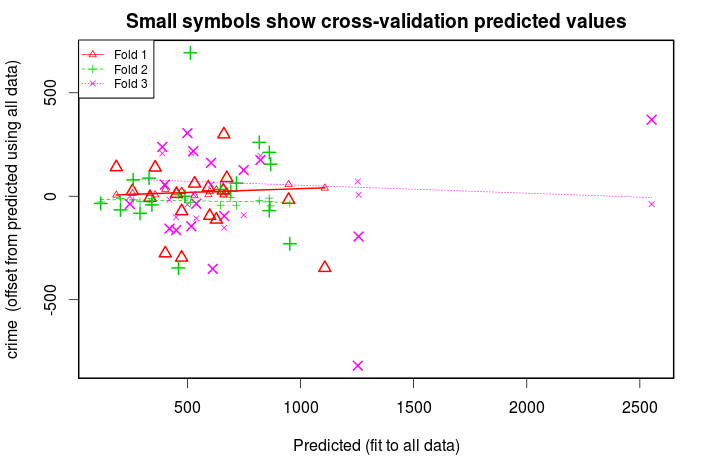
\includegraphics[width=\textwidth]{cvlm.png}
\caption{Residualplot einer 3-fachen Kreuzvalidierung mittels  Die Abszisse beschreibt die vorausgesagten Werte. Auf der Ordinate ist die Abweichung der Vorhersage zum wahren Wert des Kriteriums abgetragen, hier Gewaltdelikte pro 100'000 Einwohner.}
\label{plot:cvlm}
\end{figure}


\section{Diskussion}
Automatisierte Verfahren zur Bestimmung von Regressionsgleichungen werden eingesetzt um Modelle zu optimieren oder explorativ neue Modelle zu generieren wenn viele potentielle Prädikatoren involviert sind. 

Im Falle der Optimierung gilt es insbesondere ein zu stark an die Trainingsdaten angepasstes Modell zu vereinfachen. 
Einfachere Modelle sind in der Regel stabiler, was wiederum die Generalisierbarkeit erhöht.
Ziel ist es hierbei Prädikatoren mit geringer Vorhersagekraft zu eliminieren. Mittels exhaustiver Verfahren können sämtliche Kombinationen von den im Modell enthaltenen Prädikatoren geschätzt werden.
Aus diesem Set meist einfacherer Modelle kann mittels Kreuzvalidierung die durchschnittliche Fehlvorhersage berechnet werden. Im Idealfall wird ein einfacheres Modell gefunden, das die Daten generell besser vorhersagt als das komplexe Modell.
Der Vorteil exhaustiver Verfahren gegenüber den standardmässig eingesetzten schrittweisen Verfahren ist, dass das optimale Modell gefunden wird, insbesondere in Kombination mit der Kreuzvalidierung.
Der erhöhte Rechenaufwand sollte heutzutage nicht mehr ins Gewicht fallen, insbesondere da in der Psychologie meist nur eine Handvoll Prädikatoren ein Modell beschreiben.  

Die explorative Anwendung ist verbreiteter und dient dem schätzen von Modellen ohne klare theoretische Begründung.
Eine Auslese potentieller Prädikatoren sollte möglichst unkorreliert sein um der Multikolinearität vorzubeugen. Bei genügend grossem Stichprobenumfang und einer mässigen Anzahl an potentiellen Prädiktoren führt auch hier das exhaustive Verfahren gefolgt von einer Kreuzvalidierung zur optimalen und stabilsten Vorhersage. In der psychologischen Forschung ist der Stichprobenumfang oft knapp bemessen. Kann aufgrund des Stichprobenumfangs eine Kreuzvalidierung nicht verlässlich geschätzt werden, kommen schrittweise Verfahren zum Einsatz. Dabei werden Prädikatoren schrittweise hinzugefügt oder eliminiert, bis ein zuvor bestimmtes Kriterium nicht mehr erfüllt werden kann. Das Kriterium  besagt weshalb und wann ein Modell als akzeptabel zu betrachten ist.
Es soll ein Kriterium herbei gezogen werden, welches die Anzahl der Prädiktoren im Modell berücksichtigt um einer Überanpassung entgegen zu wirken.
Akaikes Informationskriterium als zuverlässliches Kriterium schrittweiser Regression erwiesen.  

\citeA[p. 57]{harrell2001regression} erwähnte eine ganz generelle Schwierigkeit: ``It allows us to not think about the problem.''.
Moderne leicht zu bedienende Statistikprogramme gepaart mit der Möglichkeit schier grenzenloser Rechenkapazität verführen einem nach Effekten zu fischen und \gls{glos:datamining} zu betreiben.
Der Einsatz automatisierter Verfahren zur Bestimmung von Regressionsgleichungen ist umstritten. 
Während die einen Autoren dies als ein probates Mittel ansehen lehnen andere insbesondere die schrittweise Regression ab. 
Schrittweise verfahren halten sich auch heute noch hartnäckig obschon es keinen Grund gibt nicht vollumfänglich alle Modelle durch zu rechnen. 
Die Rechenkapazität sowie die nötige Software ist vorhanden. 
Forschende sollten sich vom Gedanken lösen das Resultat gleich unmittelbar zu bekommen und dem Computer eine Kaffeepause lang die Möglichkeit geben, das optimale Resultat zu finden.
Zu guter Letzt kann man auch hier die Faustregel anwenden, dass das simpelste Verfahren das beste Resultat ergibt.

\newpage
\printglossaries 
%\addcontentsline{toc}{chapter}{Glossar}
\newpage
\bibliographystyle{apacite} 
\bibliography{literature}


\newpage
\section{Anhang}
\subsection*{Selbstständigkeitserklärung zur Literaturarbeit am  Psychologischen Institut}
\paragraph{Originalarbeit}
Ich erkläre ausdrücklich, dass es sich bei der von mir eingereichten schriftlichen Arbeit 
mit dem Titel ``Automatische Verfahren zur Prädiktorauswahl in Regressionsmodellen''um eine von mir selbst und ohne unerlaubte Beihilfe sowie in eigenen Worten verfasste 
Originalarbeit handelt. 
Sofern es sich dabei um eine Arbeit von mehreren Verfasserinnen oder Verfassern handelt, bestätige ich, dass die entsprechenden Teile der Arbeit korrekt und klar gekennzeichnet und der jeweiligen Autorin oder dem jeweiligen Autor eindeutig zuzuordnen sind.
Ich bestätige überdies, dass die Arbeit als Ganze oder in Teilen weder bereits einmal zur Abgeltung anderer Studienleistungen an der Universität Zürich oder an einer anderen Universität oder Ausbildungseinrichtung eingereicht worden ist noch inskünftig durch mein Zutun als Abgeltung einer weiteren Studienleistung eingereicht werden wird. 
 
\paragraph{Verwendung von Quellen} 
Ich erkläre ausdrücklich, dass ich sämtliche in der oben genannten Arbeit enthaltenen Bezüge auf fremde Quellen (einschliesslich Tabellen, Grafiken u. Ä.) als solche kenntlich gemacht habe. Insbesondere bestätige ich, dass ich ausnahmslos und nach bestem Wissen sowohl bei wörtlich übernommenen Aussagen (Zitaten) als auch bei in eigenen Worten wiedergegebenen Aussagen anderer Autorinnen oder Autoren (Paraphrasen) die Urheberschaft angegeben habe. 

\paragraph{Sanktionen}
Ich nehme zur Kenntnis, dass Arbeiten, welche die Grundsätze der 
Selbstständigkeitserklärung verletzen – insbesondere solche, die Zitate oder Paraphrasen ohne Herkunftsangaben enthalten –, als Plagiat betrachtet werden und die entsprechenden rechtlichen und disziplinarischen Konsequenzen nach sich ziehen können (gemäss §§ 7ff der Disziplinarordnung der Universität Zürich sowie § 36 der Rahmenordnung für das Studium in den Bachelor- und Masterstudiengängen der Philosophischen Fakultät der Universität Zürich). 

Ich bestätige mit meiner Unterschrift die Richtigkeit dieser Angaben.

Name: Markus Graf\\
Matrikelnummer:  08-91271-9\\
\\
\\
\\
\\
\\
\\
............................................................................\\
Zürich, \today



\end{document}
